\section{Data Processing Techniques}

\begin{enumerate}
    \item Image Augmentation - Importance of Augmentation in Preventing Over fitting
    \item Techniques Used (e.g., Rotation, Flipping, Zooming, Cropping)
    \item Data Preprocessing for each model VGG16, Xception, MobilenetV2
    \item Data Splitting - Training, Validation, and Test Split Ratios, Stratified Splitting to Maintain Class Distribution, Rationale for Chosen Split Ratios
    \item Handling Class Imbalance - Techniques for Managing Imbalanced Data - (e.g., Oversampling, Undersampling) Impact on Model Training and Evaluation
\end{enumerate}
\par

\subsection{Image Augmentation}
A technique used to artificially increase the training set by creating modified copies of a dataset using existing data. This technique is very useful when an image dataset is small. This also helps expose our model to different aspects of the training data and reduce overfitting. \par \vspace{1em}
We implement this process by adding an Augmentation Layer to our classifier models.
Augmentation Layer are only active during training and not during model’s inference or evaluation.\par \vspace{1em}
Our Augmentation Layer includes: RandomFlip, RandomRotation, Saturation, Brightness

\begin{figure}
    \centering
    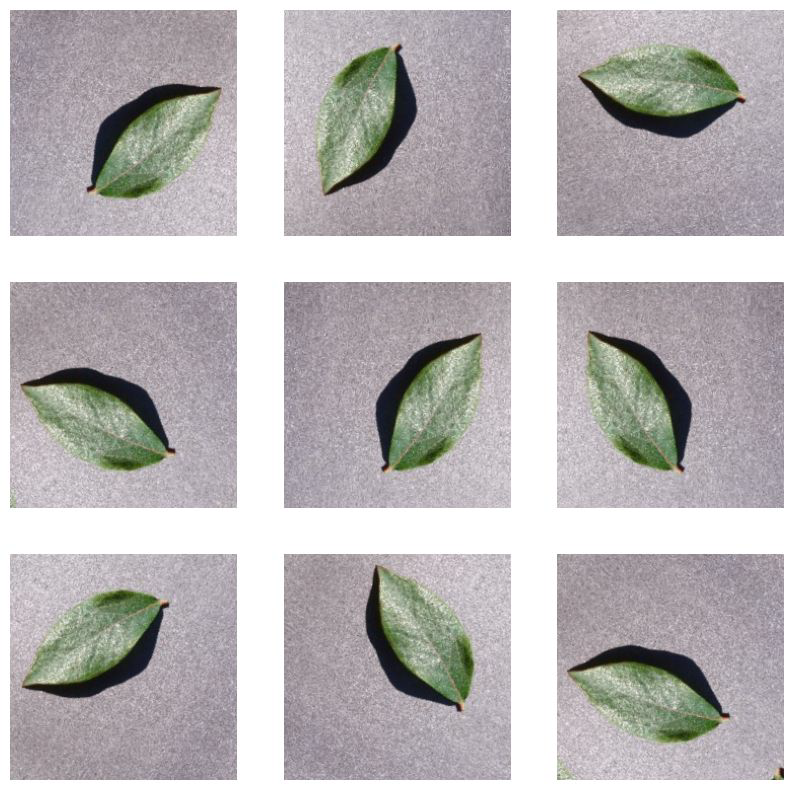
\includegraphics[width=1\linewidth]{graphics//chapter 4/image aug.png}
    \caption{Image Augmentation}
    \label{fig:img-augmentation}
\end{figure}


\subsection{Data Splitting}
The total of 10431 images are split 80:10:10, which is:\par
80\% in training, i.e. 8344 images for actual training.\par
10\% for testing, i.e. 1044 images for testing.\par
10\% for validation, i.e. 1044 images for validating the result.\par \vspace{1em}

Data Splitting is important as it helps prevent overfitting, ensure robustness and generalization.

\begin{figure}
    \centering
    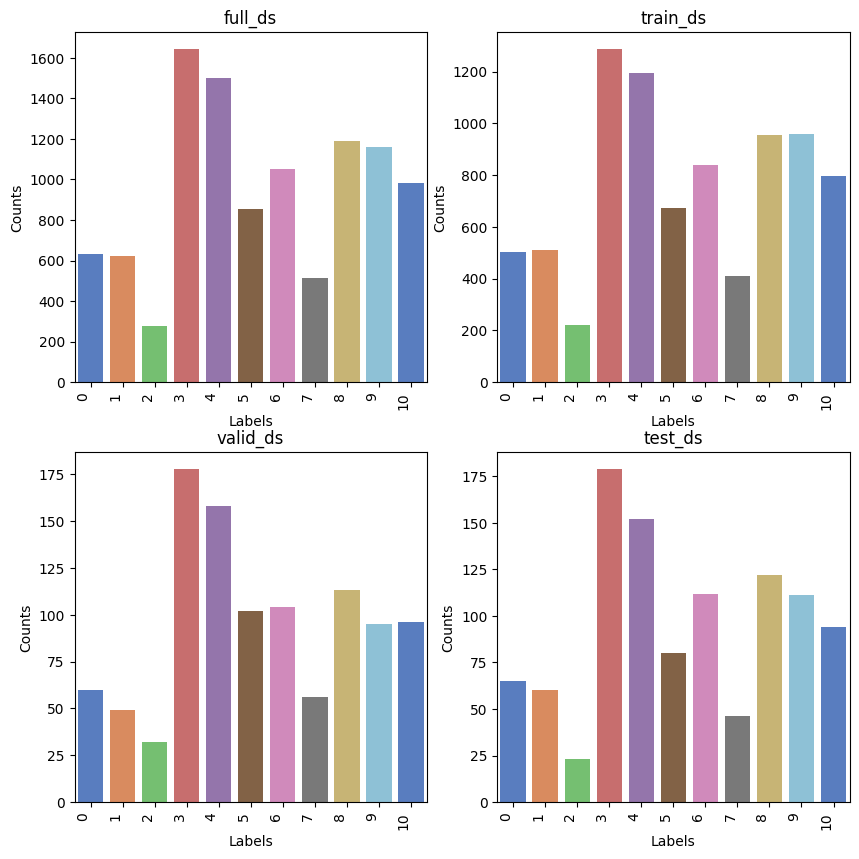
\includegraphics[width=1\linewidth]{graphics//chapter 4/train test split.png}
    \caption{Train, Test, Validation Split}
    \label{fig:train-test-split}
\end{figure}

\newpage